\newpage
\section{Scientific/Technical/Management Plan}

\subsection {Background and Motivation}

El Ni{\~n}o and Southern Oscillation (ENSO) originating in the tropical Pacific has a profound impact on the US West coastal ecosystem \citep{jacox2015enso,bograd2019water,frischknecht2015remote}. Numerous hypotheses have been proposed regarding ENSO’s effect on the US west coastal ecosystem: (i) teleconnections in the North Pacific climate, influencing coastal upwelling \citep{alexander2002atmospheric}, (ii) ocean interior processes via coastally trapped waves (CTW) that are excited in the equatorial Pacific \citep{hermann2009comparison,hickey2003local,hickey2006evolution,frischknecht2015remote}, and small scale impacts (e.g. \citep{small2014new,capet2008mesoscale,capet2004upwelling,bassin2005sub,mooers1984turbulent}).

\subsubsection{Atmospheric Teleconnections}
Atmospheric teleconnections are driven by shifts in deep convection in the tropics during different phases of ENSO, that affects the distribution and strength of the Aleutian Low pressure system, which influences changes in upwelling-favorable winds, cross-shore Ekman transports, mixed layer depth, sea surface height, temperature and salinity along the US West coast \citep{enfield1980structure,emery1985atmospheric,strub2002altimeter,checkley2009patterns}. The atmospheric teleconnections also influence the North Pacific ocean circulation as seen through Pacific Decadal Oscillation (PDO) \citep{alexander2002atmospheric,di2013synthesis}, and the North Pacific Gyre Oscillation (NPGO) \citep{di2013synthesis}, which are expressions of low frequency variability of sea surface temperatures and sea surface salinity in the North Pacific, and are linked to variations of coastal surface physical and biogeochemical properties of the Pacific Northwest coast \citep{di2009nutrient,chhak2009forcing,combes2013cross,chhak2007decadal}. 

\subsubsection{Coastally Trapped Waves}
Equatorial Kelvin waves that remotely drive CTW are generated by among other processes, Westerly/Easterly wind bursts in the western equatorial Pacific prior to an El Ni{\~n}/La Ni{\~n}a event\citep{mcphaden1988response,eisenman2005westerly,chiodi2014subseasonal,chen2015strong,fedorov2015impact}, often due to the Madden Julian Oscillation \citep{chen1996multiscale,feng2018assessing,yang2019upscale}.   The wind bursts excite downwelling/upwelling waves, which suppresses/shoals the equatorial thermocline as it propagates eastward, and northward along the North American coast covering a distance of 11,000 km in a month \citep{thomson2010poleward,engida2016remote}. As the CTW travels, a downwelling Kelvin wave suppresses the isopycnals, deepens the thermocline, and raises the sea level, whereas an upwelling wave does the opposite, shoaling the isopycnals, bringing cooler subsurface waters. 

\subsubsection{Small scale influences}
In addition to large scale changes in winds associated with shifts in the Pacific North American and PDO patterns, smaller scale winds are known to be important to coastal upwelling (e.g., \citep{small2014new,capet2004upwelling}).  These small scale winds imprint highly variable wind stress curl on the ocean that is not captured in most models, as well as most observational products.  Small scale variations in wind stress and CTW propagation can lead to the formation of mesoscale eddies (e.g. \citep{lorenzo2004modelling}).  These eddies can have profound impacts on coastal and ecosystem dynamics (e.g. \citep{correa2007mesoscale}).

Upwelling will lead to increases in horizontal buoyancy gradients off shore.  These gradients are susceptible to instability and submesoscale eddies (e.g. \citep{fox2008parameterization}) often form.  These have been seen in observations and models for the California Current System (CCS, e.g. \citep{capet2008mesoscale}).  These submesoscale eddies can have strong restratifiying effect (slumping isopycnals) on the upper ocean \citep{fox2011parameterization} as well as nutrient distributions \citep{brannigan2016intense}.  Near the coast these eddies have length scales of between 5-10 km, making them difficult to observe and model.

The processes described above can have profound effects that vary strongly on intra- and inter-annual timescales.  Further these processes can act in isolation or in concert making their affects on coastal dynamics and ecosystems difficult to assess.  All of these processes as well as different water masses from the eastern equatorial Pacific will influence the CCS \citep{bograd2019water,thomson2010poleward,bograd2015changes,meinvielle2013decadal} via the California Undercurrent (CUC). 

\subsection {California Undercurrent} 

All eastern boundary upwelling systems include a poleward flowing, subsurface current called an undercurrent.  In the case of the CCS, the poleward flowing California Undercurrent (CUC) transports warm and salty Pacific Equatorial Water (PEW) to the Aleutian Islands, covering an incredible distance of 11,000 km, affecting the physical and bio-geochemical properties of the shelf and slope waters along its path on the US West coast \citep{reed1976observations,thomson2010poleward,connolly2014coastal,meinvielle2013decadal,nam2015seasonal,hickey2016alongcoast}. The CUC is an important component of the California Current System, and along with CTW, contributes to the remote alongshore oceanic advection of equatorial source waters that affects the seasonal predictability of shelf waters. The CUC traverses mostly along the upper slope with offshore extent varying seasonally and with latitude.  The CUC strengthens during late summer to fall in the Northern CCS (N-CCS), and contributes towards large scale along coast advection that affects the mid-shelf bottom water, and upper slope water in the region \citep{stone2018effect,hickey2016alongcoast} including temperature and salinity both seasonally, interannually and decadally. Several studies have linked the slope properties or presence of the CUC to shelf properties along the CCS \citep{thomson2010poleward,meinvielle2013decadal,turi2018,durski2017influence}.
Changes in mixing, stratification, and depth of the isopycnal associated with the CUC influences the coastal upwelling on the shelf. The depth of the CUC core determines the upwelled water properties along the shelf and slope more than the composition of the water transported by CUC in recent observational and modeling work, \citep{meinvielle2013decadal,stone2018effect}.  Despite its importance to the CCS, current global climate models have a difficult time resolving the properties of the CUC including its seasonal development (Figure~\ref{fig:CUC}), mostly due to their coarse resolution \citep{hickey2016alongcoast}. 

\begin{figure}[h]
  \centering
  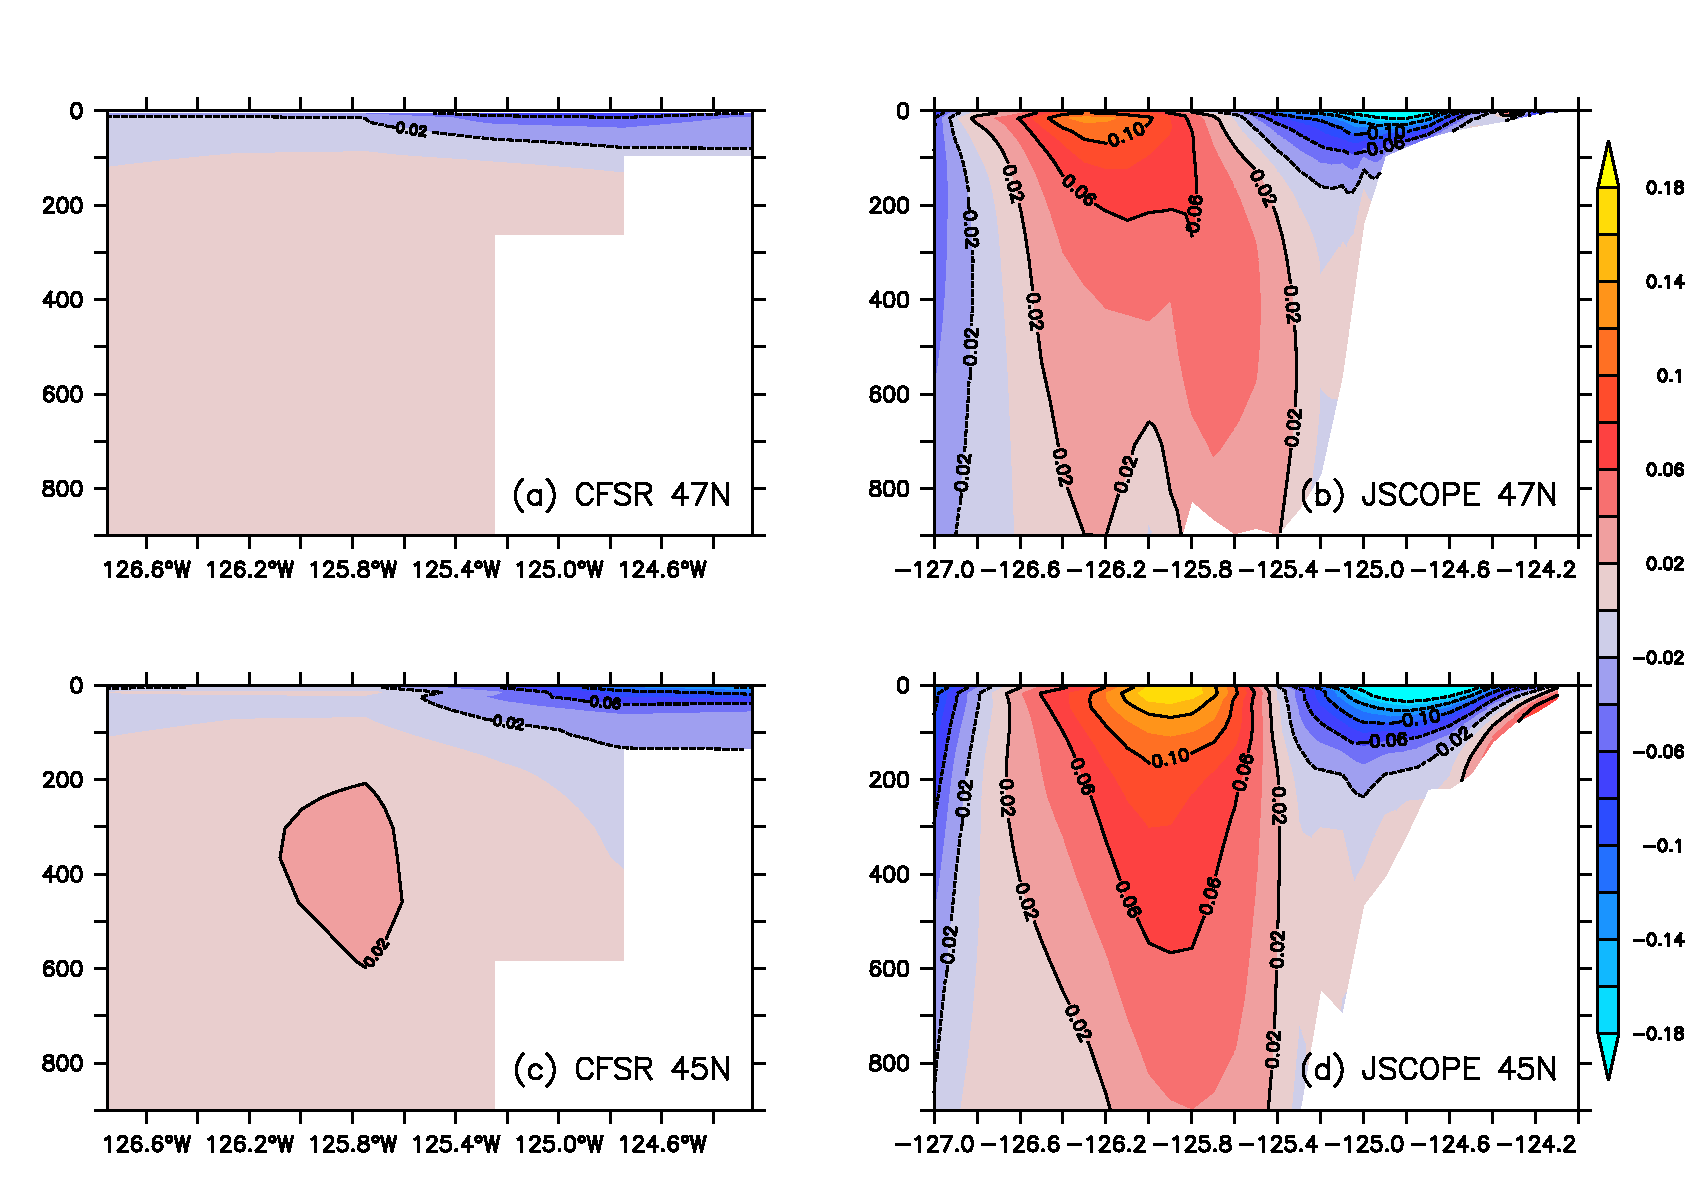
\includegraphics[width=0.8\textwidth]{CUC_obs_CFSR.pdf}
  \caption{Longitudinal transects of meridional velocity (m/s) from (left) CFSR (NCEP's CFS reanalysis \citep{saha2010ncep} using MOM4 version 4p0d \citep{griffies2004technical} with a horizontal resolution of 25-50 km, and a 10m spacing in the upper 200m) compared to (right) J-SCOPE  (JISAO's Seasonal Coastal Ocean Prediction of the Ecosystem \citep{siedlecki2016experiments} using downscaled ROMS in Cascadia domain  with a horizontal spacing of 1.5 km and 40 vertical levels) simulations at (top) 47N and (bottom) 45N averaged for the month of August over the period 2009-2017. Red (blue) shading represents poleward (equatorward) current. Shading is every half a contour. Note, the poleward current on the shelf bottom at 45N in J-SCOPE that CFSR fails to resolve.}
  \label{fig:CUC}
\end{figure}

To model the CUC correctly, it is important to capture the northward energy transport associated with CTW \citep{connolly2014coastal} and thus the CUC core is modulated by a propagating CTW \citep{connolly2014coastal,stone2018effect}. Further, given that the CUC exists very close to the coastal shelf, and its seasonal variability along the shelf, the biogeochemical and bathymetric details of the shelf and slope needs to be accurately represented in current generation of climate models \citep{durski2017influence,thomson2010poleward,hickey2016alongcoast,bograd2019water}.   This is difficult to do in present climate models as this requires very high resolution globally, making the simulations very computationally expensive. Regional downscaling using a high resolution configuration of the Regional Ocean Model shows a migration of the poleward current in early fall onto the coastal shelf, potentially affecting the stratification and the upwelling.  Current climate models with coarse resolution fail to capture the phenomena (Figure~\ref{fig:CUC}))  

On longer timescales, preliminary work by Co-I Ray has shown that the depth of the CUC in CFSR reanalysis shows decadal variability mostly south of 45N, and interannual variability along the entire CCS mostly following strong El Ni{\~n}o events. Further, analysis shows a deepening of the CUC core following El Ni{\~n}o events in CFSR (Figure~\ref{fig:CUC_enso}).  While the CUC in coarse resolution models is weaker than observed, the presence of it is promising in terms of mechanistic pathways of diagnosing and understanding signals for ENSO-driven variability along the CCS, and its contribution to seasonal predictability of ocean conditions within the CCS. 


\begin{figure}[h]
  \centering
  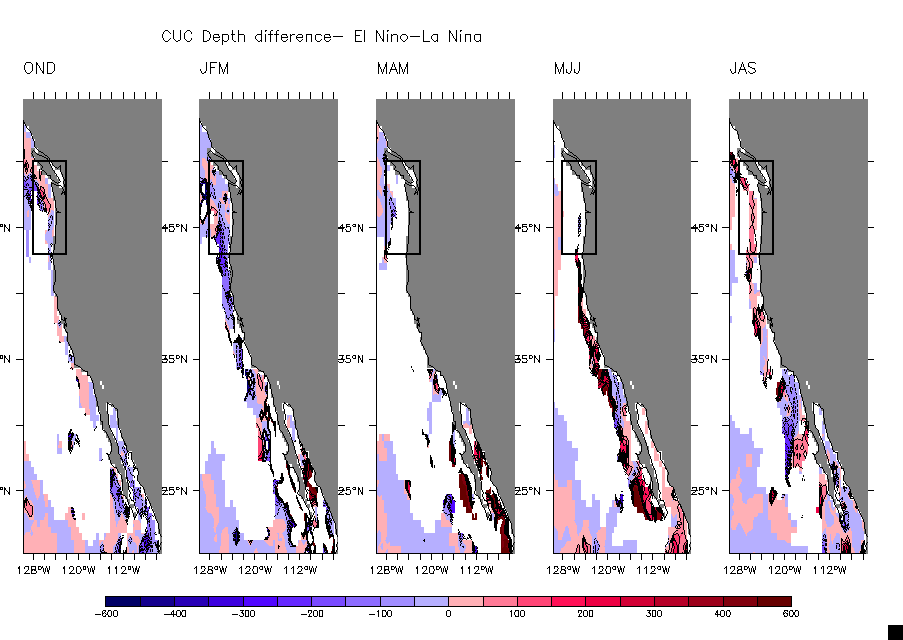
\includegraphics[width=0.8\textwidth]{CUCdepth_difference_EL_LA.png}
  \caption{Horizontal maps of the difference in the depth (m) of the maximum poleward current (representative of the CUC core), averaged in each season following an El Ni{\~n}o and a La Ni{\~n}a event. Composites of 10 El Ni{\~n}o and 8 La Ni{\~n}a events are shown for the period 1979-2017 from CFSR simuation. OND is for 0 year, and JFM, MAM, MJJ, JAS are for +1 ENSO year. Red (blue) shading indicates deeper CUC core in El Ni{\~n}o (La Ni{\~n}a). Note, the deeper core of the CUC in the following MJJ, and JAS season of El Ni{\~n}o. }
  \label{fig:CUC_enso}
\end{figure}

Thus, to understand physical mechanisms and pathways of connection between tropical Pacific and coastal upwelling and dynamics (including longer timescale variability) along the US West coast, we must understand the processes that influence the CCS and the CUC.  This is complicated as a single process can dominate or multiple processes can operate at once.  Diagnosing and understanding these coastal features is imperative to understand the impact of the ENSO generated signal on the west coast of the United States, which to the best of our knowledge has not yet been explored. 

\subsection{Research Questions}
While numerous questions remain to fully understand mechanisms connecting the tropical variability to coastal upwelling, via CTW, and CUC -its strength and variability, here we focus on the following questions:
\begin{itemize}
    \item [\textbf{Q1}-] What are the relative impacts of local versus remote processes on CUC and upwelling variability?
    \begin{itemize}
        \item We expect fluctuations in along shore windstress and pressure gradients to control the CUC locally
        \item Remotely generated CTW from the equator could impact CUC depth and variability, mostly during ENSO.
        \item Locally generated eddies will modify local density gradients and upwelling and hence CUC variability
        \item CTW is an essential source of energy for CUC to show up  along the coastal shelf 
    \end{itemize}
    \item [\textbf{Q2}-] How are the local and remote processes that act on the CUC modified by different types of El Ni\~no events, e.g. dateline vs East Pacific events?
    \item [\textbf{Q3}-] What is the role of tropical synoptic variability on coastal teleconnections?
    \begin{itemize}
        \item Does MJO matter for the ENSO connection to coastal upwelling?
        \item Based on the relation of westerly wind bursts on different types of El Ni\~no, how does that affect CTW propagation?
    \end{itemize}
\end{itemize}

\section{Expected Impact and Relevance}

The proposed work directly addresses the call by using state estimates and in-situ data to understand ocean variability (in this case CUC variability and its connection to the equatorial Pacific).  The work combines two existing NASA state estimates from the Estimating the Circulation and Climate of the Ocean (ECCO) project to assess the variability and magnitude of the CUC and also isolate the climatological impacts of mesoscale eddies on CUC variability.  We will also utilize the Energy Exascale Earth System Model (E3SM), which contains variable resolution capabilities in all components, to attempt to quantify the role of submeso and mesoscale variability in fully coupled configurations.  These new analyses will lead to new insights on the role of small scale processes in CUC variability, leading to a better prediction of upwelling, which could lead to improved fidelity of long term projections of marine ecosystem health and marine heat waves \citep{oliver2018longer,heidemann2019marine}.

The work also addresses CLIVAR goals of understanding the role of the ocean in climate variability (coastal upwelling), quantifying uncertainty in model projections, and understanding processes that govern climate variability.  Further, our simulations could lead to predictive relationships between coastal upwelling and in situ quantities (e.g. temperature/salinity/chlorophyll/wave height).  If the statistical relationships are robust, and the critical variables are not observed presently it could suggest future directions for NASA measurement missions.  Relatedly, our E3SM results could show a strong dependence on flow structures in the ocean at small scales $< 25$ km.  This may also suggest directions for future measurement missions.  The influence of coupled dynamics on relationships could also suggest future directions for the ECCO project.

\section{Technical Approach}

To begin to disentangle these complex processes and their interactions we propose to examine a heirarchy of state estimates, and model simulations.  Some processes, such as mesoscale eddy distributions in the CCS and correlations with ENSO could be diagnosed with satellite data (e.g. Surface Altimetery, REFNEEDED, or high resolution sea surface temperature, GHRSST, REF).  However, it is likely that these products do not have high enough temporal resolution to sufficiently resolve processes like CTWs, but can provide a climatological effect of eddy processes on the CCS.

The bulk of our approach utilizes a heirarchy of state estimates and targeted model simulations (Section~\ref{sec:heirarchy}).  Through all of the analysis we will include a new analysis developed by Co-I Ray (Section~\ref{sec:heatBudget}) that has led to an improved understanding of the Pacific Equatorial Cold Tongue \citep{ray2018understanding}.

\subsection{A model and state estimate hierarchy}
\label{sec:heirarchy}

To answer our key research questions, we must isolate and filter processes to quantify process impact.  We propose a separation in space, and configuration.  The easiest separation is achieved in space, where we can consider data products and state estimates and different resolutions to isolate the impacts of mesoscale eddies.  CTWs are well resolved in numerous climate model configurations and can be diagnosed at near $1^\circ$ resolution.  However, resolution of the northward coastal current is difficult at low resolution (Figure~\ref{fig:E3SM_meridVel}).  Most of the processes described in Section 1 are modified by coupling between the atmosphere and ocean.  To assess this modification we can utilize models in different spatial and forcing configurations.  In this effort, we propose to utilize the ECCO and ECCO2 state estimates and the E3SM model.

\begin{figure}[h]
  \centering
  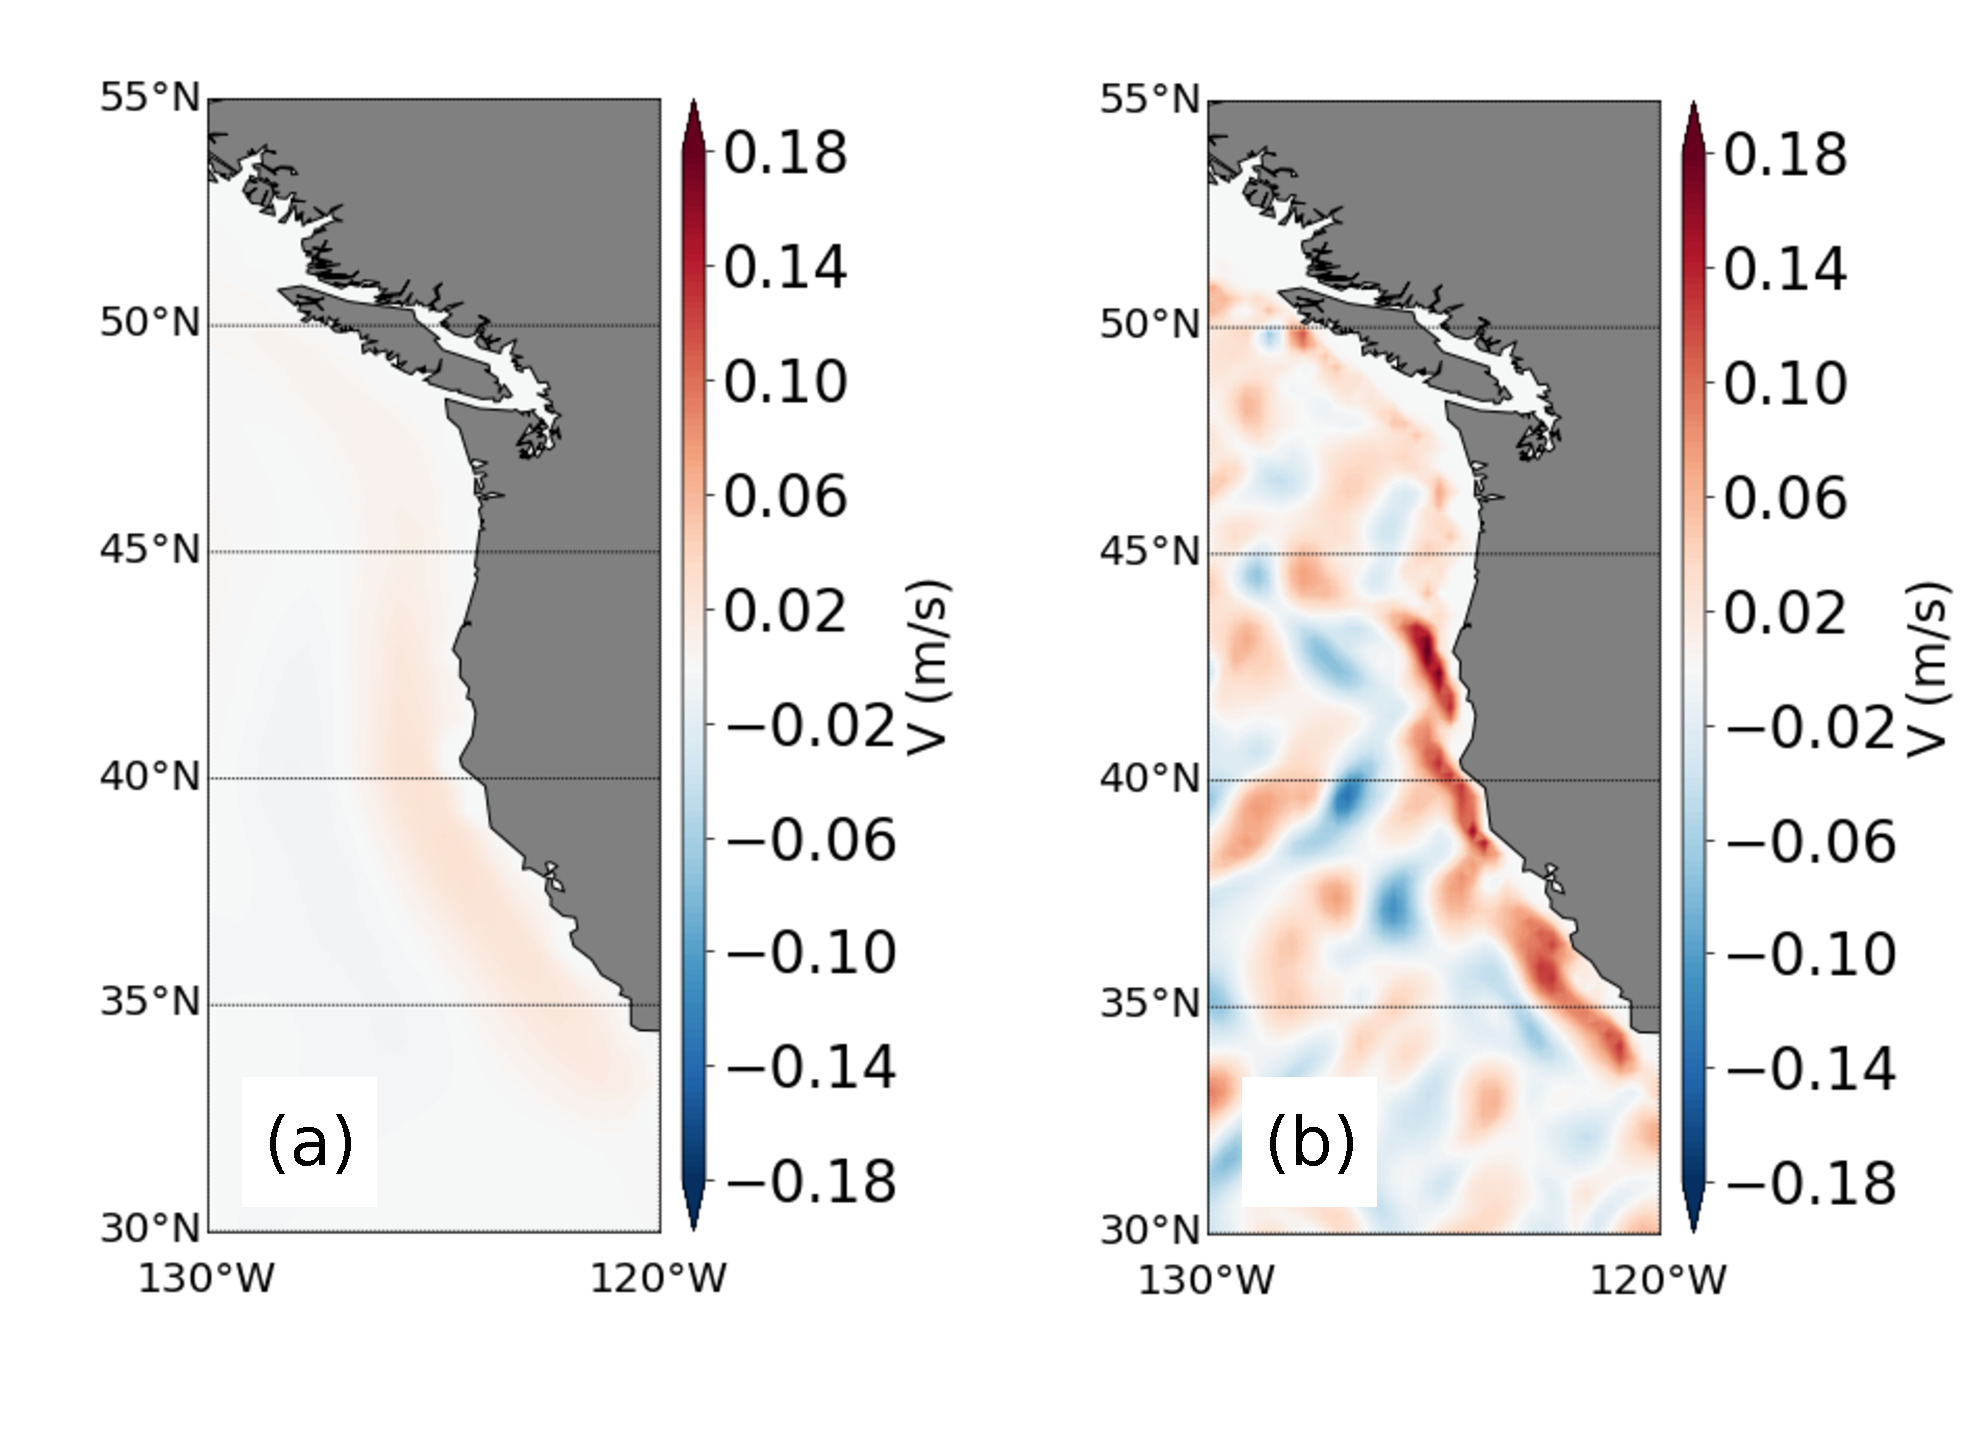
\includegraphics[width=0.8\textwidth]{e3smmeridcurrent.eps}
  \caption{Horizontal maps of August meridional velocity at 300m depth in fully coupled E3SM simulations following the Highres MIP protocal (HAARSMA REF NEEDED) at low resolution (a) and high (eddy resolving) resolution (b).  The model output is averaged between years 40-50 of the simulations.}
  \label{fig:E3SM_meridVel}
\end{figure}

\subsubsection{ECCO and ECCO2 State Estimates}
\color{red}
\begin{itemize}
    \item fix citations
\end{itemize}
\color{black}

The ECCO project \citep{forget2015} is a data assimilated ocean state estimate, that includes data from ARGO, Satellites like GRACE, TOPEX/Poseidon, and Aquarius.   The fit to climatological data for v4 of ECCO has greatly improved relative to previous releases.  However, this product will not include the impacts of some of the critical processes discussed above (e.g. submeso and mesoscale eddies).  ECCO2 \citep{menemenlis2005using,menemenlis2005nasa} is the first eddy resolving ocean sea-ice assimilated state estimate.  Both ECCO and ECCO2 utilize the MITgcm \citet{marshall1997finite} as the dynamical ocean. The ocean model is coupled to a sea-ice model that computes ice thickness, ice concentration,and snow cover as per \citet{zhang1997efficient} and that simulates a viscous-plastic rheology.  

The horizontal resolution of ECCOv4 is approximately one degree globally, except at the equator where the resolution increases to 1/3 degree.  The ECCO2 product utilizes a cubed sphere discretization \citep{adcroft2004implementation} with a mean global resolution of 18km.  Both models are forced at the surface by data products; at low resolution ERA-Interim is primarily used \citep{forget2015} and in ECCO2 the ECCO simulation, extrapolated to high resolution through a Green's function approach \citet{menemenlis2005using} is used as a boundary condition \citet{menemenlis2005nasa}.  The dataset from ECCO and ECCO2 cover the period 1992-2015 and can thus be used to understand our research questions.  Although, given the short period the results may not be robust.

Given that the atmosphere used in both ECCO and ECCO2 is not interactive, we are unable to quantify how atmosphere-ocean coupling modifies the processes discussed in Section 1.  Further, the low temporal frequency of the data products used to force the ocean, we also preclude assessing the influence of intraseasonal forcing of CTW by the Madden Julian Oscillation (REFS NEEDED).  Therefore we require model simulations to more completely assess the role of ENSO oceanic teleconnections on CUC and upwelling strength and variability.

\subsubsection{E3SM}
\color{red}
\begin{itemize}
    \item fix refs
\end{itemize}
\color{black}
E3SM version 1 (hereafter E3SMv1) began from a branch of the Community Earth System Model version 1 \citep{hurrell2013community}. While much of the infrastructure for performing simulations and coupling processes is unchanged, the component models have either undergone massive modification or have been replaced entirely. Ocean and sea-ice components are now based on the Model for Prediction Across Scales \citep{ringler2013multi,petersen2019evaluation}. MPAS-Ocean uses a energy and mass conserving, finite volume discretization on a staggered C-grid \citep{Arakawa77,thuburn_numerical_2009,ringler2013multi}. Tracer advection is via a quasi 3rd-order, three-dimensional, flux corrected transport scheme \citep{Skamarock_Gassmann11jcp}.  A z-star vertical coordinate within an Arbitrary Lagrangian-Eulerian scheme is used, where the all layer thicknesses in a column expand and contract with the sea surface height \citep{petersen_evaluation_2015,reckinger_study_2015}.  At non eddying resolutions, the Gent McWilliams \citep{gent1990isopycnal} eddy parameterization is used.   Notably, at high resolution uses an increased number of vertical layering designed to more accurately simulate the vertical structure of mesoscale eddies \citep{stewart2017vertical}.  This is in contrast to the relatively coarse 10m upper layers of E3SM low resolution and both ECCO products.  

MPAS-Seaice replicates the \citet{Hunke1997} Elastic-Viscous-Plastic numerics on our hexagonal mesh. Sea ice column physics are described in \cite{golaz2018doe} and are very different from their CESM1 predecessor: e.g., Sea ice thermodynamics were changed from the \cite{bitz1999} enthalpy-conserving method to \cite{turner2015} mushy-layer physics with prognostic brine drainage. CESM virtual melt ponds \citep{Holland_et12} were replaced with the explicit level-ice pond scheme of \cite{hunke2013}.

In the atmosphere, the stratiform microphysics scheme is upgraded to the prognostic double-moment parameterization of \cite{Gettelman_Morrison15, Gettelman_et15}. Treatment of shallow convection are all replaced by the comprehensive Cloud Layers Unified By Binormals scheme \citep{Golaz_et02, Larson_Golaz05, Larson_17}. A spectral-element dynamical core is applied, as described in \cite{Dennis_et12}. The \cite{Zhang_McFarlane95} deep convection scheme is unchanged relative to CESM1, but a number of its parameters have been retuned in v1 \citep{Xie_et18,Rasch_et19,golaz2018doe}.  A simple linearized ozone photochemistry scheme \citep{Hsu_Prather09} is used to predict ozone changes. 

As noted in \cite{golaz2018doe}, the ocean model in E3SMv1 accounts for changes in heat content of water with temperature, but the atmosphere does not. Keeping track of water heat content in the atmosphere is challenging, so E3SMv1 instead applies an ad hoc correction where the global-average difference between the temperature at which water evaporates from the ocean and returns back as rain or stream outflow is applied as a globally-uniform sensible heat flux correction. This correction was found to have negligible effect on model climate and is described in more detail in \cite{golaz2018doe}, their Appendix A.   

\subsubsection{E3SM Model Configurations}
\color{red}
\begin{itemize}
    \item fix refs
\end{itemize}
\color{black}

Presently the E3SM project has run numerous simulations at climate resolution ($1^\circ$ atmosphere and land and ocean ice resolution of 30 km near the equator and poles and 60km in the midlatitudes - see \citet{petersen2019evaluation} or \citet{golaz2018doe}), with nearly 2000 years of simulation data available.  At high resolution ($0.25^\circ$ atmosphere and land and ocean ice resolution of 18km at the equator and 6km near the poles), 50 years have been run following the highresMIP protocol \citep{haarsma2016high}, which is a 1950 control integration.  Initial analysis suggests a few important features: (1) ENSO is consistent with observations (See \citet{golaz2018doe} their Figure 20) and (2) the representation of the Madden Julian Oscillation also compares very well with observations\citep{golaz2018doe}.  This data is publicly available on the Earth System Grid Federation (ESGF; \url{https://esgf-node.llnl.gov/projects/e3sm/}) and will be used to analyze mechanisms of CUC variability.  When these are contrasted against our ECCO and ECCO2 analysis we can begin to assess the influence of atmosphere-ocean coupling.  However, there are a few important caveats.  First, the dynamical models in ECCO and E3SM are completely different and a direct comparison is difficult.  To mitigate this we will also analyze CORE2 forced \citep{large2009global} simulations with E3SM (at resolutions similar to ECCO and ECCO2) to quantify how coupling effects change in E3SM and between E3SM and ECCO.  Second, in each analysis we are analyzing a single realization of climate only.  It is therefore difficult to differentiate emergent signals and oceanic teleconnections from internal model variability.  To quantify internal E3SM variability we will collaborate with the E3SM large ensemble project currently underway (PI Van Roekel is a collaborator on that project at present).

While the presently (and soon to be) available simulations will constraiin pathways between equatorially generated CTWs and CUC variability we propose to design model meshes that can effectively separate  the impacts of remote versus local impacts on the CUC.  This is similar to the regional data assimilation method \citep{lu2016understanding,lu2017understanding} where outside of a focus region (our high resolution zone) the solution is either nudged or assimilated to data.  With a naturally transitioning mesh, we can easily transition nudging on and off.  Further, we effectively filter high resolution processes from lower resolution regions.  Initially we will utilize the coastally enhanced mesh, which was designed for the upcoming E3SM simulation campaign (an earlier version is shown in Figure~\ref{fig:coastalMesh}, the newest version enhances resolution around Greenland).

\begin{figure}[h]
  \centering
  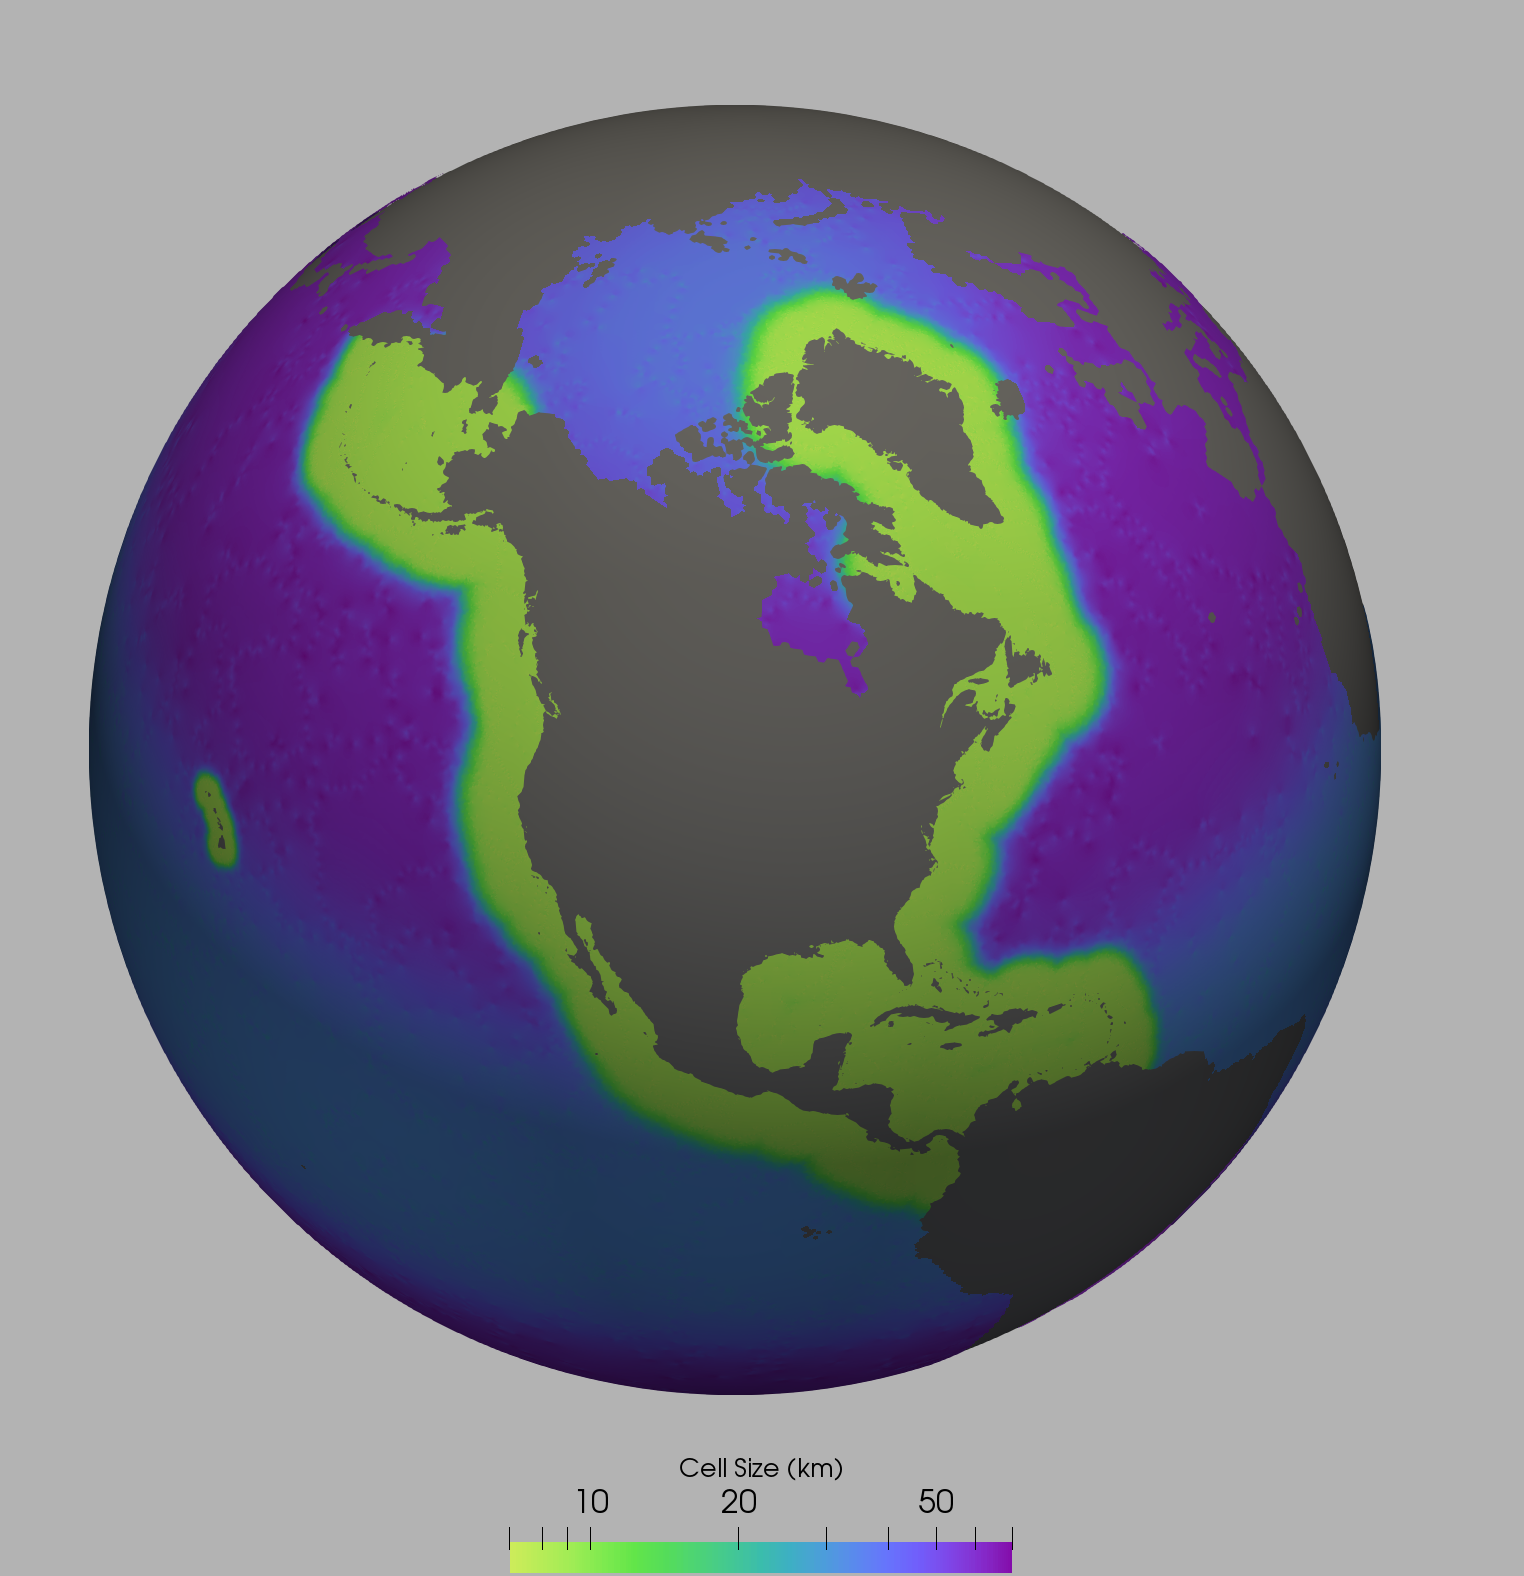
\includegraphics[width=0.6\textwidth]{cellSize.png}
  \caption{Map of cell size for the proposed ocean and ice grid.  Resolution in the green area is 8km and outside of the transition zone the mesh is identical to the low resolution E3SM configuration.}
  \label{fig:coastalMesh}
\end{figure}

Our coastally enhanced mesh exhibits a greatly improved northward current (Figure~\ref{fig:E3SM_CONUS_meridVel} compare to Figure~\ref{fig:E3SM_meridVel}).  The simulation now bears many similarities to the global high resolution simulation, albeit with a slightly weaker CUC.  This weaker signal is likely due to the low resolution atmosphere, as previous research \citep{capet2004upwelling,small2014new} suggests high resolution winds are required to correctly simulate coastal dynamics.  This benefit is realized at roughly 1/8 the cost of the high resolution simulation.  This mesh will be utilized and will allow us to create a number of E3SM realizations that simulate at least some of the critical coastal ocean processes not well simulated at low resolution.

\begin{figure}[h]
  \centering
  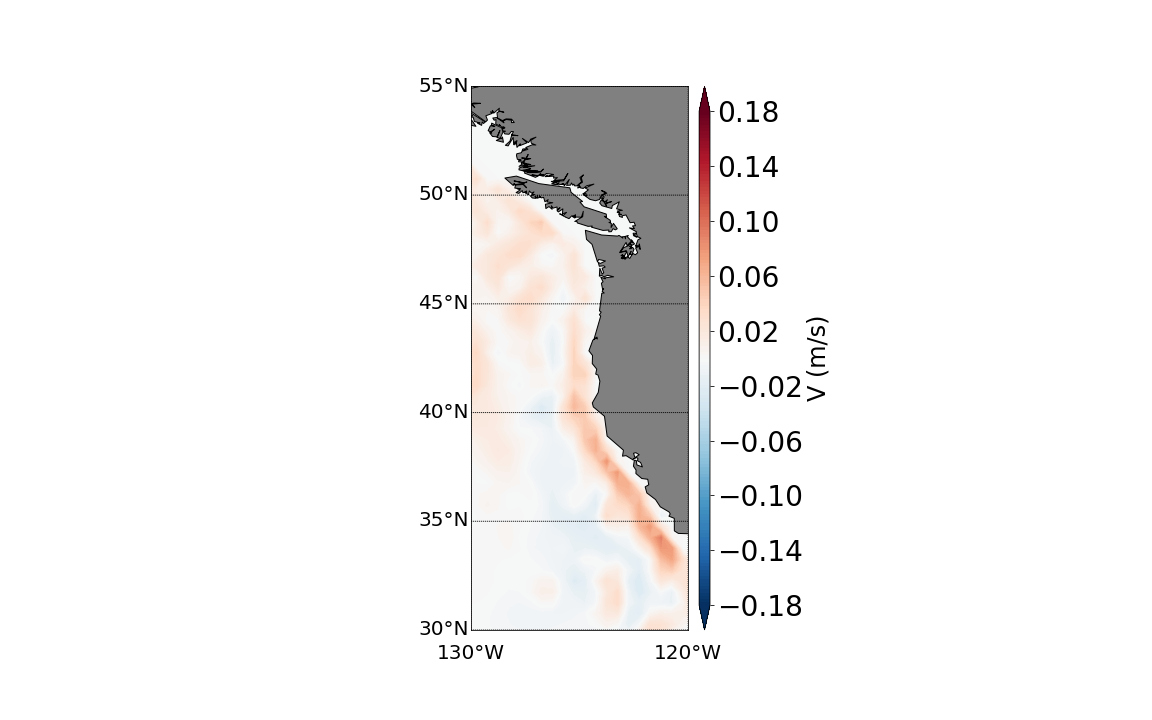
\includegraphics[width=0.8\textwidth]{meridionalVelocity_300m_CONUS_aug.png}
  \caption{As in Figure~\ref{fig:E3SM_meridVel} but for the coastally enhanced mesh (Figure~\ref{fig:coastalMesh}).}
  \label{fig:E3SM_CONUS_meridVel}
\end{figure}

In the last year of the project we will extend the coastal enhanced mesh to attempt to simulate the impact of frontal filamentation and submesoscale eddies \citep{capet2008mesoscale} on CUC variability for the first time.  In these simulations we propose to remove the enhancement near the arctic and embed a ultra high resolution in the CCS region (similar to \citep{lorenzo2004modelling}).  This will allow for minimal increases in horizontal degrees of freedom, however, the simulation will be more costly due to the concomitant reduction in model timestep.  We plan to run these simulations seasonally with initial conditions drawing from interpolated E3SM HR simulations.

\subsection{Analysis Plans and Tools}
 
 Analysis of this complex problem will involve a variety of standard analysis (e.g. autocorrelation, EOF), but we will also leverage key analysis available within MPAS and one recently developed by CO-I Ray.
 
\subsubsection {Heat-Budget diagnostics}
\label{sec:heatBudget}

The Pacific Northwest off the Washington/Oregon shelf and the equatorial Pacific cold tongue in the eastern Pacific are similar regions where the CUC and the EUC shoals respectively, creating a layer of highly stratified water column with intense mixing in the upper ocean. The core of the CUC and EUC control the upwelling and vertical mixing in these regions respectively. It is well known that current generation of climate models have a hard time simulating the equatorial Pacific cold tongue. To understand this bias,  \citet{ray2018understanding} develops a framework to summarize the equatorial Pacific upper ocean temperature budget, which are compatible with the CMIP6 output variable list. This framework analyzes the diurnal, seasonal, and interannual variations of the equatorial cold tongue temperature budgets revealing key roles of the net surface heat flux (at diurnal and interannual scales), resolved advection (at submonthly, seasonal, and interannual scales), and parametrized vertical mixing (at diurnal, seasonal, and interannual scales; Figure~\ref{fig:heatBudget}). Using this framework \citet{ray2018understanding,ray2018evaluation} show that the strong cooling of the surface mixed layer due to advection and vertical diffusion during boreal autumn of La Ni{\~n}a years due to lack of adequate stirring from Tropical Instability Waves (TIWs) could be a key contributor to the excessive equatorial cold tongue in GFDL-FLOR global climate model. Given the similarity of the CUC and EUC regions and the generality of the framework, we intend to use this methodology to calculate the advective fluxes via CUC and EUC in the Pacific Northwest and eastern equatorial Pacific regions, in particular their variabilities on interannual timescales, and quantify their impact on the coastal upwelling.
We will also asses the interannual variability in the zonal advective fluxes via EUC and the meridional advective fluxes via CUC. 

\begin{figure}[h]
  \centering
  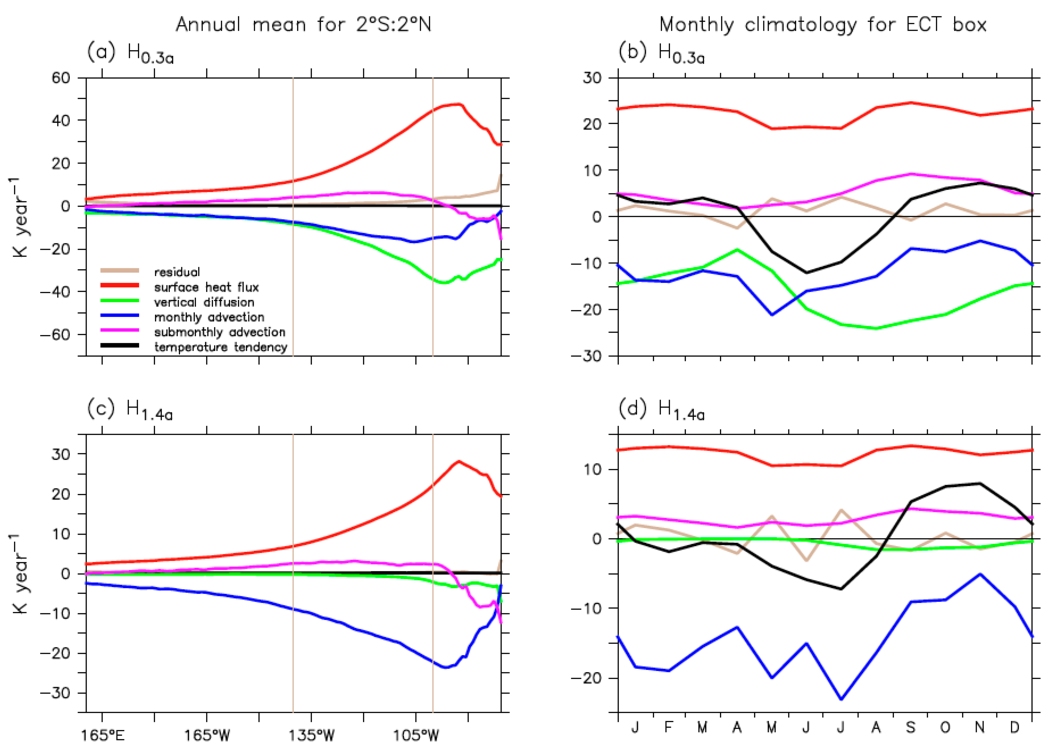
\includegraphics[width=0.8\textwidth]{heatBudget.pdf}
  \caption{Model simulated layer temperature budgets for (left) the $2^\circ$S to $2^\circ$N band as a climatological annual mean, and (right) the cold tongue region as a 12 month climatology.  The budget extends vertical over (a),(b) the surface mixed layer and (c),(d) the advective layer.  Colors indicate the net surface heat flux minus shortwave penetrating through the layer base (red), parameterized local diffusion due to vertical mixing (green) and monthly advection (blue), all submonthly advection including subdaily advection (magenta), and the sum of all remaining terms (gray).  Vertical lines in (a) and (c) show the zonal extent of the cold tongue box.}
  \label{fig:heatBudget}
\end{figure}

\subsubsection{in situ E3SM analysis}
At high resolutions, it can often be difficult to analyze mode output.  Significant time must be spent in writing data to disk from the model and then reading it into analysis routines.  In addition, it is not feasible to store all the three-dimensional fields desired for analysis.  To make analysis more efficient, MPAS includes a number of in situ analysis routines that operate on data as the model is running while data is in memory.  Previous work \citep{woodring2015situ} has shown this approach to be more efficient than conducting analysis after the model run is complete.  Here we will leverage a number of important MPAS analysis routines.  First, MPAS calculates a full tracer budget that is closed for each timestep and cell as well as for any geographic region.  Second, we will utilize the high performance lagrangian particle tracking analysis \citep{wolfram2015diagnosing} that will help visualize variations in the CUC.

\subsection{Uncertainties and Risk Mitigation}
\color{red}
\begin{itemize}
    \item Where appropriate we have discussed risk, we utilize pre-existing simulations and data as much as possible also our work plan proceeds in parallel to allow the simulation design for year 3 to begin early and not interfere with other tasks.
\end{itemize}
\color{black}

The ECCO and model analysis each contain a few uncertainties that could hinder progress.  As an example, TOPEX/Poseidon and other altimetry data may filter out shorter timescales, making diagnosis of CTW pathways difficult.  Analysis of other, higher frequency data sources (e.g. TAO/TRITON buoys).  Further, the analysis of model simulations allo us to explicitly control the what fields are output and their respective frequencies.  In our model analysis, development of a new mesh is not without inherent risk.  This has led us to first analyzing the newly developed mesh for the E3SM project, that has already been rigorously tested.  Finally, the new submesoscale resolving mesh, which has the most risk, can be developed in parallel to all other tasks.  Further, the tools used to generate MPAS meshes has become quite robust and easier to use recently, greatly reducing risk associated with the generation of a new mesh.

\section{Team Member Roles}

PI Van Roekel will lead the overall project effort, arrange and hold project meetings, and ensure that all deliverables are met.  His primary expertise is in ocean turbulence through large eddy simulation across a very wide range of scales (isotropic turbulence to the mesoscales) and parameterization of vertical turbulent fluxes of heat, momentum, and salt for large scale ocean models.  Recently he has worked to understand ENSO variability in E3SM and this work has led to large reduction in tropical variability biases in the model.  Parts of this work are documented in \citep{golaz2018doe}.  He has also successfully used E3SM in an ultra high resolution configuration (submesoscale resolving), albeit in an idealized (annular) configuration.  He will also be responsible for acquiring all necessary computational resources for the project.  Van Roekel has a long track record of acquiring computational resources.  To date his work has successfully leveraged nearly 500 million cpu hours, where most hours were acquired through competitive proposals.  Note also that Los Alamos National Laboratory features a number of advanced computational platforms (detailed in Appendix~\ref{sec:facilities}).  These resources are available through a separate proposal process and can be acquired at no cost to this budget.

Although Van Roekel is only listed as 10\% on the proposal, the questions we are pursing in this proposal would are important considerations for the E3SM project, but cannot be pursued as a part of that project.  Therefore another $\approx 25\%$ of Van Roekel's ()who is also the co-lead of the water cycle science campaign for E3SM) E3SM time will be leveraged as in-kind support of this project.

In the first year of this proposal PI Van Roekel will hire a unnamed post doctoral researcher at LANL.  This postdoc will lead the development of the ultra high resolution mesh and conduct the simulations on Los Alamos computational resources.  Approximately 50\% of the LANL postdoc funding will come from this budget.  The other 50\% will be funded through internal LANL programs, such as the Center for Space and Earth Sciences \url{https://www.lanl.gov/projects/national-security-education-center/space-earth-center/index.php}

The work at the University of Connecticut will be led primarily by Co-I Ray.  She has recently designed a novel methodology for heat budget analysis (summarized in Section~\ref{sec:heatBudget}) that has been used to develop new understanding for mechanisms governing equatorial cold tongue variability.  This is a general methodology that can be used in various regions and models.  She has demonstrated analysis expertise and will lead the analysis during the project.

Finally, Co-I Siedlecki is the current mentor of Co-I Ray.  Although she is not a funded participant of the project, she has expertise in coastal physics and bogeochemistry and will continue to mentor Co-I Ray on this project and will provide her expertise in an advisory capacity to the project as a whole.

\section{Timeline}

\begin{figure}[h]
	\centering
	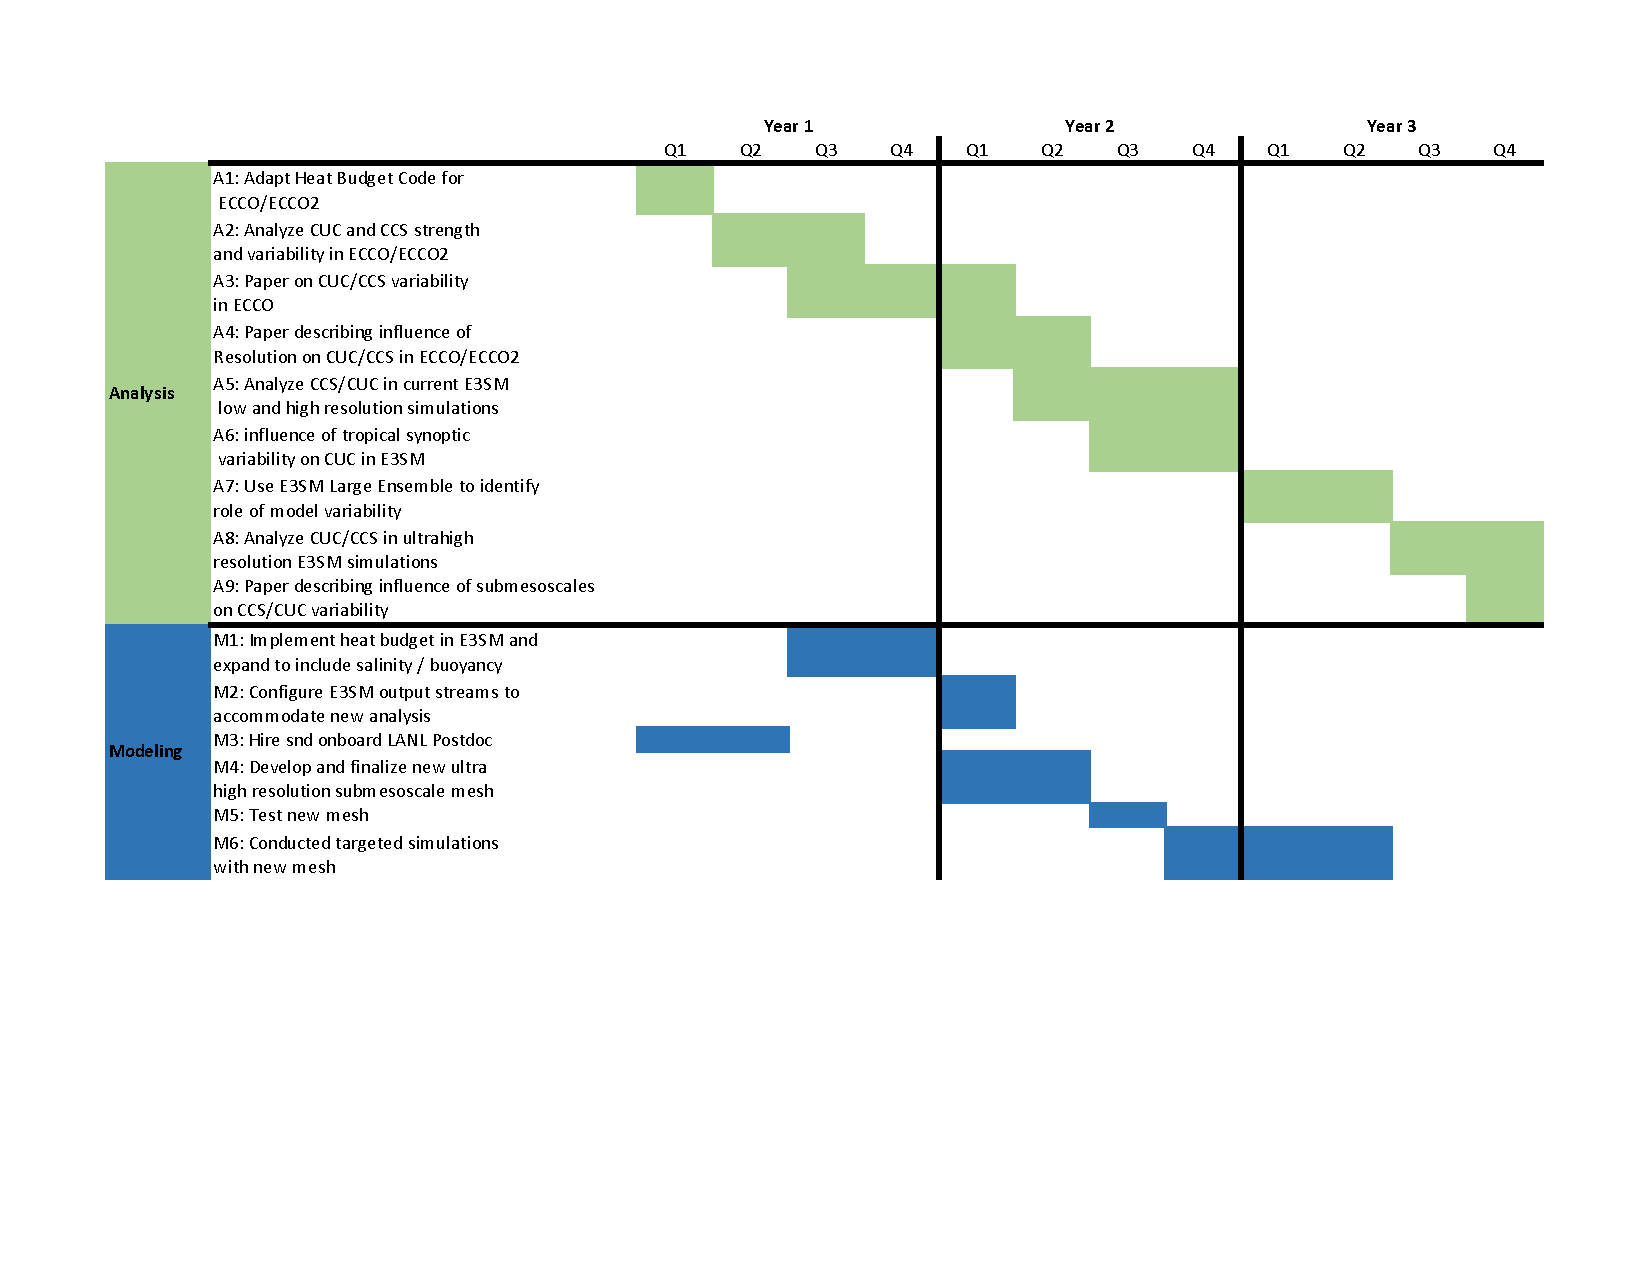
\includegraphics[width=1\textwidth]{Timeline_NASA.pdf}
\end{figure}


\section{Management Plan}


\begin{itemize}

    \item 50\% postdoc to be funded at LANL, with other 50\% coming from other sources at LANL
    \item SS - lead UConn PI will provide coastal expertise and "advise" SR on the project
    \item SR - implement heat budget code within E3SM and analyze ecco and ecco2 products.
    \item SR and LANL PD to combine to configure and run new e3sm simulations.
\end{itemize}

Rough timeline
\begin{itemize}
    \item Year 1 - analyze ECCO and ECCO2 data to assess mechanisms of CUC variability on ENSO timescales, with particular focus on the role of resolution -- i.e. filter the high res data to reemove the mesoscales and compare to ECCO Low res.  Hire LANL PD and have new PD work with SR to implement heat budget analysis for E3SM data.
    \item Year 2 -- analyze e3sm high res /low res and new coastally enhanced resolution simulations to see the influence of localized resolution versus global and high versus low resolution.  Led by LANL PD with help from SR.   Also start to configure regionally ultra high resolution (~1km) simulations on west coast.
    \item Year 3 -- run and analyze the ultra high res simulation.  Summarize findings.
\end{itemize}
